\documentclass[12pt, a4paper]{report}
\usepackage{graphicx}% LaTeX package to import graphics
%\graphicspath{{images/}} % configuring the graphicx package
\usepackage{amsmath}
\usepackage{float}
\usepackage{pgfplots}
\usepackage{pgfplotstable}
\usepackage{subcaption}
\usepackage{listings}
\usepackage{tabularx}
\usepackage[margin=2cm]{geometry}
\lstset{basicstyle=\ttfamily}

\begin{document}
\setlength{\baselineskip}{0.5cm}

\begin{titlepage}
    \centering
    
    \Huge\textbf{Analysis of Deep Learning Architectures for Accurate Covid 19 Detection from CT Scan Images}
    
    \vspace{1cm}
    
    \Large\textbf{Project Report}
    
    \vspace{1cm}
    
    \large\textbf{Presented by :}
    
    \textbf{Nakka Vishnu Vardhan}\\
    \textbf{Ritu Raj Prasad}\\
    \textbf{Vemulapadu Sai Puneeth Reddy}
    \vspace{1cm}
    
    \large\textbf{Project Guide :}
    
    \textbf{Dr.Sanath Kumar Tulasi}
    
    \vspace{1cm}
    
    \textbf{Date:}
    
    \textbf{April 16, 2024}\
    \\
    \vspace{1cm}
    
\includegraphics[width=0.5\textwidth]{report images/image1.png}

    \vspace{.4cm}
    
    \large\textbf{Department of Electronics and Communication Engineering}\\
      \vspace{.4cm}
    \textbf{National Institute of Technology, Andhra Pradesh}
    
\end{titlepage}

\newpage

\chapter*{Declaration}
\addcontentsline{toc}{chapter}{Declaration}

We declare that this written submission represents our ideas in our own words and where others' ideas or words have been included, we have adequately cited and referenced the original sources. We also declare that we have adhered to all principles of academic honesty and integrity and have not misrepresented or fabricated or falsified any idea/data/fact/source in our submission. We understand that any violation of the above will be cause for disciplinary action by the Institute and can also evoke penal action from the sources which have thus not been properly cited or from whom proper permission has not been taken when needed.

\vspace{2cm}

\begin{tabular}{@{}l l l@{}}
    \textbf{NAKKA VISHNU VARDHAN} & 621217 & DATE:16/04/2024 \\
    \textbf{RITU RAJ PRASAD} & 621240 & DATE:16/04/2024 \\
    \textbf{SAI PUNEETH REDDY VEMULAPADU} & 621242 & DATE:16/04/2024 \\
\end{tabular}

\newpage

\chapter*{Acknowledgements}
\addcontentsline{toc}{chapter}{Acknowledgements}

We would like to share our sincere gratitude to our supervisor \textbf{Dr. Sanath Kumar Tulasi} for helping us in completion of this project. During the work we faced many challenges as the field is new and due to our lack of knowledge and experience, but he helped us to get over from all the difficulties and in final completion of our project. We have learnt many new things during the project discussion. We are really glad to be associated with a person like Dr. Sanath Kumar Tulasi. All of our team is thankful to all department faculty members for their support.\\

We profoundly thank \textbf{Dr. Yuvaraj S}, Head of ECE department who has been an excellent guide and also a great source of inspiration to our work. We would like to acknowledge the help for giving us all the required permissions and helping us to complete the project. We would like to thank all the faculty of the ECE department for teaching us and for spending time for the review. We also thank our friends who directly or indirectly helped us in our project work and completion of the report in time. Lastly, we would like to thank our families for their selfless support.

\vspace{1cm}

\begin{flushright}
    \textbf{Nakka Vishnu Vardhan}\\
    \textbf{Ritu Raj Prasad}\\
    \textbf{Vemulapadu Sai Puneeth Reddy}
\end{flushright}


\newpage

\chapter*{Abstract}
\addcontentsline{toc}{chapter}{Abstract}

In the wake of the COVID-19 pandemic, accurate and efficient diagnosis of the virus remains paramount. Computed Tomography (CT) scans have emerged as a valuable tool for detecting COVID-19 due to their sensitivity in revealing characteristic pulmonary abnormalities associated with the disease. Deep Learning (DL) techniques have shown promising results in automating COVID-19 diagnosis from CT images. However, selecting the most effective DL architecture is crucial for achieving high accuracy and generalization.\\

This project aims to analyse various DL architectures for COVID-19 detection from CT scan images. We propose to investigate convolutional neural network (CNN) architectures such as Alex Net, VGG, along with advanced models like U-Net and Attention mechanisms tailored for medical image analysis. The study will encompass a comprehensive evaluation of these architectures on a large dataset of COVID-19 CT scans, comparing their performance in terms of accuracy, sensitivity, specificity, and computational efficiency.\\

Moreover, transfer learning techniques will be explored to leverage pre-trained models on large-scale image datasets, adapting them to the task of COVID-19 detection. The project will also investigate data augmentation strategies to enhance model robustness and mitigate over-fitting, considering the limited availability of annotated COVID-19 CT scan datasets.\\

Furthermore, interpretability of DL models will be addressed to provide insights into the features learned by the networks, aiding clinicians in understanding the decision-making process. Attention will be given to explainable DL techniques such as Grad-CAM and saliency maps to visualize regions of the CT scans crucial for COVID-19 diagnosis.\\

Through rigorous experimentation and analysis, this project aims to contribute to the development of accurate and reliable DL-based systems for COVID-19 detection from CT scan images, facilitating timely diagnosis and patient management in the ongoing battle against the pandemic.


\newpage

\tableofcontents

\newpage

\listoffigures

\newpage

\chapter{Introduction}
\addcontentsline{toc}{chapter}{Introduction}

The COVID-19 pandemic, caused by the novel corona virus SARS-CoV-2, has posed
unprecedented challenges to global public health systems, economies, and societies. As the world continues to grapple with the evolving crisis, effective diagnosis and management of COVID-19 cases remain critical in controlling the spread of the virus and mitigating its
impact on human health.\\

Amidst the diverse array of diagnostic tools available for COVID-19 detection, Computed Tomography (CT) imaging has emerged as a valuable adjunct to reverse transcriptionpolymerase chain reaction (RT-PCR) testing, particularly in cases where RT-PCR results are inconclusive or unavailable. CT scans can reveal characteristic pulmonary abnormalities associated with COVID-19, such as ground-glass opacities, consolidations, and bilateral lung involvement, aiding in the timely identification and triaging of suspected cases.\\

However, the manual interpretation of CT scans for COVID-19 diagnosis is labour-intensive, time-consuming, and subject to inter-observer variability. The growing demand for rapid and accurate diagnosis has spurred interest in leveraging artificial intelligence (AI) and Deep Learning (DL) techniques to automate COVID-19 detection from CT images. DL models, particularly convolutional neural networks (CNNs), have demonstrated remarkable capabilities in medical image analysis, surpassing human performance in certain tasks.\\

In this context, this project endeavours to explore and analyse various DL architectures tailored for COVID-19 detection from CT scan images. By harnessing the power of DL, we aim to develop robust and accurate models capable of assisting clinicians in the rapid identification and classification of COVID-19 cases from CT scans. Through a systematic evaluation of different DL architectures, transfer learning strategies, and interpretability techniques, we seek to advance the state-of-the-art in automated COVID-19 diagnosis and contribute to the ongoing efforts to combat the pandemic.

\section{Introduction to Deep Learning}
\vspace{0.25cm}

Deep learning, a powerful branch of artificial intelligence, mimics the human brain's structure and function. It utilizes artificial neural networks, layered like the brain, to learn from vast amounts of data. These layers progressively extract intricate patterns from images, text, or sounds. By training on this data, deep learning models can be programmed to perform remarkable tasks like recognizing objects in photos or translating languages. Essentially, it allows computers to learn and improve without needing every step explicitly coded, making it a revolutionary tool for artificial intelligence.

\subsection{Enhancement of AI}

In the modern era, AI is rapidly advancing across various domains such as deep learning, natural language processing, and computer vision. These advancements enable improved healthcare diagnostics, financial decision-making, and industrial automation. AI's ethical considerations, including bias mitigation and transparency, are increasingly prioritized. Additionally, AI contributes to addressing global challenges like climate change through
predictive modelling and environmental monitoring. Overall, AI's evolution drives transformative changes, necessitating responsible development and deployment for societal benefit.

\subsection{Need of Deep Learning}

Deep learning is essential for handling complex data patterns, enabling more accurate predictions and insights. Its hierarchical structure allows for automatic feature extraction, reducing the need for manual feature engineering. This technology powers advancements in fields like image recognition, natural language processing, and autonomous systems. Deep learning's scalability and adaptability make it crucial for analysing vast datasets efficiently. Its role in driving innovation across industries underscores its significance in the modern era.

\section{Introduction to CNN}
Convolutional Neural Networks (CNNs) are a class of deep neural networks designed for processing structured grid-like data, such as images. They utilize convolutional layers to automatically learn hierarchical patterns and features from input data. CNNs are widely used in computer vision tasks, including image classification, object detection, and facial recognition. Their ability to capture spatial dependencies and translational invariance makes them highly effective for analysing visual information. CNNs have revolutionized various applications, from medical imaging to self-driving cars, by achieving state-of-the-art performance in complex visual tasks.

\begin{figure}[htbp]
    \centering
    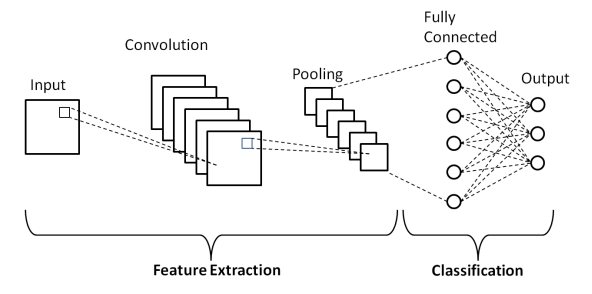
\includegraphics[width=1\textwidth]{report images/image2.png}
    \caption{\textit{Convolutional Neural Network}}
\end{figure}
\subsection{Introduction to Neural Networks}
Neural Networks are computational models inspired by the human brain's structure and function. They consist of interconnected nodes organized in layers, where each node processes and transmits information. Through a process called training, neural networks learn to recognize patterns and make predictions from input data. They're widely used in machine learning for tasks such as classification, regression, and pattern recognition. Neural networks have revolutionized fields like image recognition, natural language processing, and robotics with their ability to learn complex relationships from data.\\

\begin{figure}[htbp]
    \centering
    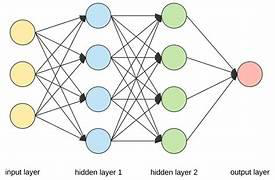
\includegraphics[width=1\textwidth]{report images/image3.png}
    \caption{\textit{Simple Neural Network}}
\end{figure}

\subsection{CNN over ANN}
Convolutional Neural Networks (CNNs) excel over traditional Artificial Neural Networks (ANNs) in tasks involving grid-like data, such as images or sequences. CNNs leverage specialized layers for feature extraction, enabling them to capture spatial hierarchies efficiently. They reduce the number of parameters by sharing weights, making them computationally efficient for large-scale datasets. CNNs inherently consider local spatial correlations, allowing them to achieve superior performance in tasks like image classification, object detection, and image segmentation. This specialization makes CNNs the preferred choice for tasks where spatial relationships and feature hierarchies are crucial, outperforming ANNs in many computer vision applications.

\subsection{Advantages}
\begin{itemize}
    \item \text CNNs automatically learn hierarchical representations of data, capturing spatial patterns and features at different levels of abstraction.This hierarchical approach is well-suited for tasks like image recognition, where features at different scales are crucial.
    \item \text CNNs use parameter sharing, where a small set of weights is reused across different parts of the input data. This reduces the number of parameters, making the model more efficient and easier to train, especially for large datasets.
    \item \text CNNs are inherently translation invariant, meaning they can recognize objects regardless of their position in the input image. This property is crucial for tasks like object detection and classification, where the location of objects may vary.
    \item \text Convolutional layers in CNNs are designed to automatically extract relevant features from input data, reducing the need for manual feature engineering. This capability makes CNNs highly effective for tasks like image recognition and segmentation.
\end{itemize}

\subsection{Applications}
\begin{itemize}
    \item \text CNNs are extensively used for image classification tasks, where they can accurately categorize images into predefined classes. Applications include identifying objects in photos, medical image diagnosis, and quality control in manufacturing.
    \item \text CNNs excel in object detection tasks,locating and classifying objects within images or videos. This application is vital for tasks such as autonomous driving, surveillance systems, and industrial inspection.
    \item \text CNNs are employed in semantic segmentation tasks to classify each pixel in an image into specific categories, enabling detailed understanding of image content. This is crucial for applications like medical image analysis, autonomous navigation, and scene understanding in robotics.
    \item \text CNNs are utilized for facial recognition systems, accurately identifying and verifying individuals from images or video frames. These systems find applications in security, access control, and personalized user experiences in various digital platforms.
    \item \text CNNs are also applied in NLP tasks such as text classification, sentiment analysis, and document categorization. They can effectively process text data by treating it as a sequence of tokens, contributing to advancements in chatbots, language translation, and content recommendation systems.
\end{itemize}

\section{Introduction to COVID 19}
COVID-19, caused by the novel coronavirus SARS-CoV-2, is a highly contagious respiratory illness that was first identified in Wuhan, China, in December 2019. It has since evolved into a global pandemic, affecting millions worldwide. The virus spreads primarily through respiratory droplets when an infected person coughs, sneezes, or talks. Common symptoms include fever, cough, and difficulty breathing, with severe cases leading to pneumonia and
organ failure. Public health measures such as wearing masks, social distancing, and vaccination campaigns have been implemented globally to control the spread of the virus and mitigate its impact on healthcare systems and economies.

\subsection{Causes and Effects of COVID 19}
COVID-19, caused by the novel coronavirus SARS-CoV-2, has had profound effects
globally. Originating in Wuhan, China, in late 2019, the virus quickly spread worldwide through respiratory droplets, leading to a pandemic. Its health effects range from mild symptoms like fever and cough to severe respiratory distress and organ failure, with certain populations at higher risk. Healthcare systems faced unprecedented challenges, with shortages of medical supplies and overwhelmed facilities. Societal and economic impacts included job losses, business closures, and disruptions to education and daily life.
Governments and organizations implemented measures like testing, vaccination, and public health guidelines to mitigate the spread and lessen the pandemic's toll on health and society.

\subsection{Step of AI in Detection}

Artificial intelligence (AI) has emerged as a powerful tool in detecting COVID-19 by leveraging advanced data analysis techniques. Initially, AI systems collect and preprocess large datasets comprising medical images such as X-rays and CT scans, clinical data, and epidemiological information. Deep learning models like Convolutional Neural Networks (CNNs) then analyse medical images to identify characteristic patterns indicative of COVID19 infection, aiding in accurate diagnosis. Furthermore, AI-powered clinical decision support systems assist healthcare professionals by integrating symptoms, medical history, and laboratory results to enhance diagnostic accuracy. AI-driven epidemiological models predict the spread of COVID-19, enabling policymakers to implement effective containment measures. Additionally, AI expedites drug discovery and vaccine development by screening
compounds, simulating interactions, and identifying potential candidates. Overall, AI plays a pivotal role in augmenting the detection, management, and prevention of COVID-19 through its ability to extract actionable insights from diverse datasets.

\subsection{Importance of CT Scan Images in Detection}
CT scan images are essential in COVID-19 detection through Convolutional Neural Networks (CNNs) due to their ability to visually represent lung abnormalities like groundglass opacities and consolidations. These images complement PCR testing by revealing lung damage, especially in asymptomatic or early-stage cases. CNNs analyze CT scans rapidly, aiding in efficient screening and early intervention during outbreaks. They provide quantitative analysis for objective disease assessment, assisting in clinical decision-making. Additionally, AI-powered CNNs enable remote diagnosis and triage, reducing healthcare burden and exposure risks.

\section{Introduction to Standard Architectures}
\subsection{LENET Architecture}
LeNet, a pioneering convolutional neural network (CNN) architecture, comprises seven layers: two convolutional layers followed by max-pooling layers and fully connected layers. In the convolutional layers, filters convolve with input images, followed by the application of activation functions like the hyperbolic tangent (tanh). Max-pooling layers reduce spatial dimensions by selecting the maximum value in each region. Fully connected layers perform a dot product with weight matrices and add biases, followed by activation functions. These layers implement mathematical operations such as convolutions, pooling, and matrix multiplications with nonlinear activations, enabling feature extraction and classification.

\begin{figure}[htbp]
    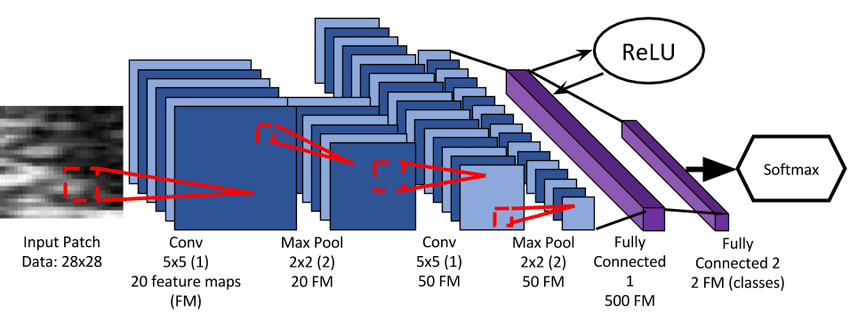
\includegraphics[width=1\textwidth]{report images/image4.png}
    \caption[LENET Architecture]{\textit{LENET Architecture}}
\end{figure}

\subsection{VGG16 Architecture}
VGG-16 is a deep convolutional neural network (CNN) architecture consisting of 16 layers, primarily composed of convolutional layers and fully connected layers. Each convolutional layer applies multiple filters to the input image, followed by rectified linear unit (ReLU) activation functions. Max-pooling layers reduce spatial dimensions, preserving important features. The fully connected layers perform matrix multiplications with learned weights and biases, followed by ReLU activations. VGG-16's mathematical operations involve
convolutions, pooling, matrix multiplications, and nonlinear activations, enabling hierarchical feature extraction and classification.

\begin{figure}[htbp]
    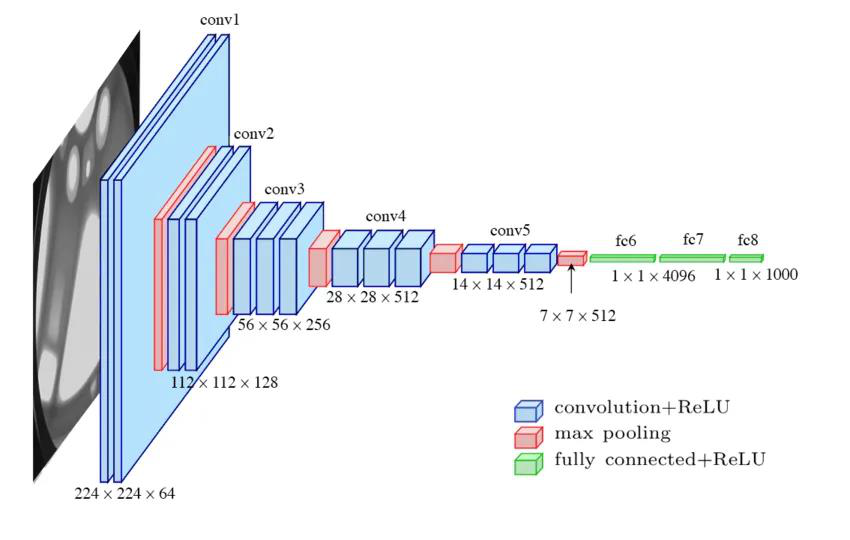
\includegraphics[width=1\textwidth]{report images/image5.png}
    \caption[VGG16 Architecture]{\textit{VGG16 Architecture}}
\end{figure}

\subsection{ALEXNET Architecture}
Alex Net is a deep convolutional neural network (CNN) architecture consisting of 5 convolutional layers followed by 3 fully connected layers. Each convolutional layer applies filters to the input image, followed by rectified linear unit (ReLU) activations. Max-pooling layers down sample feature maps, preserving important information. The fully connected layers perform matrix multiplications with learned weights and biases, followed by ReLU
activations. Alex Net’s mathematical operations include convolutions, pooling, matrix multiplications, and nonlinear activations, facilitating hierarchical feature extraction and classification.

\begin{figure}[htbp]
    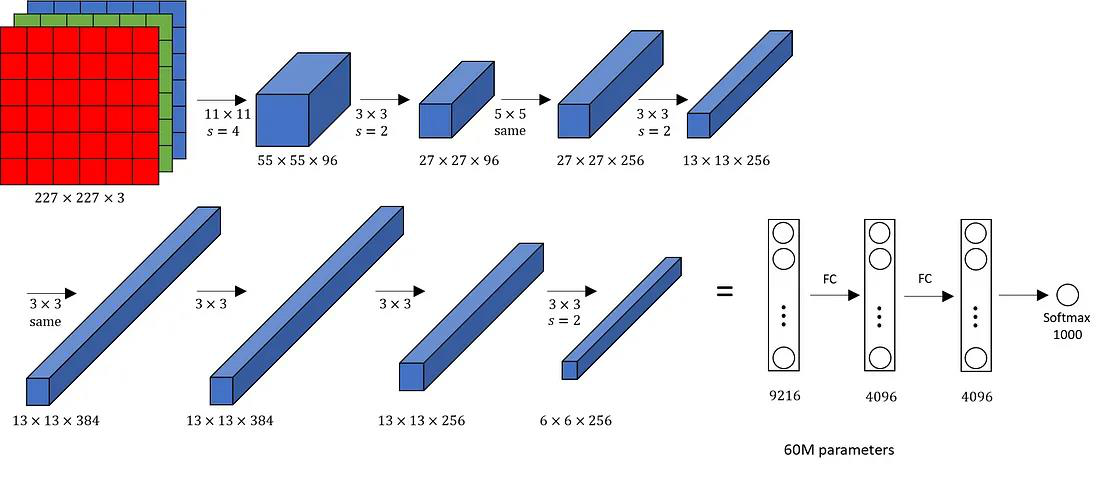
\includegraphics[width=1\textwidth]{report images/image6.png}
    \caption[ALEXNET Architecture]{\textit{ALEXNET Architecture}}
\end{figure}


\chapter{Literature Survey}
The paper which was taken as reference was published in the journal Expert Systems with Applications, volume 204, in 2022. This research paper compares the performance of 21 different convolutional neural network (CNN) architectures in detecting COVID-19 from chest X-ray (CXR) images using the COVIDx8B dataset. The COVIDx8B dataset is a large and heterogeneous COVID-19 CXR dataset with 16,352 images from patients in at least 51 countries.\\

The paper first provides background on the importance of early COVID-19 detection, the limitations of the commonly used RT-PCR testing, and the potential of using CXR images and deep learning methods like CNNs for COVID-19 diagnosis. It also reviews related work on applying CNNs to COVID-19 detection from CXR images, noting that most prior studies used smaller and more homogeneous datasets compared to COVIDx8B.\\

The 21 CNN architectures tested include popular models like VGG, ResNet, DenseNet, and EfficientNet. All models were initialized with weights pre-trained on the ImageNet dataset and fine-tuned on the COVIDx8B dataset. The training, validation, and test subsets were defined by the dataset authors to ensure no patient overlap between the sets.\\

The paper presents the results of the individual CNN models on the test set, reporting accuracy, sensitivity (TPR), precision (PPV), and F1 score. The best individual model was DenseNet169, achieving 98.15 percent accuracy and 98.12 percent F1 score. Other top-performing models included EfficientNetB2, InceptionResNetV2, and InceptionV3.\\

To further improve the classification performance, the paper explores creating ensembles of the CNN models. It first combines different top-performing models, and then creates ensembles of multiple instances of the same model (e.g., 5 instances of DenseNet169). The ensemble of 5 DenseNet169 models achieved the highest accuracy of 99.25 percent and F1 score of 99.24 percent, outperforming the previous state-of-the-art results on the COVIDx8B dataset.\\

The paper also provides a detailed analysis of the results on the training, validation, and test subsets separately. It notes that accuracy and sensitivity tend to be higher on the training and validation sets compared to the test set, while precision is higher on the test set.\\

It provides a comprehensive comparison of 21 CNN architectures for COVID-19 detection on the large and diverse COVIDx8B dataset, with results averaged over multiple training runs to account for the stochastic nature of neural networks. It demonstrates the effectiveness of CNN ensembles, particularly multiple instances of the top-performing DenseNet169 model, in achieving state-of-the-art performance on the COVIDx8B dataset. It offers insights into the dataset characteristics and their impact on the model performance across the training, validation, and test sets, highlighting the importance of handling class imbalance in such medical imaging tasks.\\

The findings of this research can guide future work on developing robust and reliable deep learning-based COVID-19 detection systems from CXR images, which can complement the limitations of RT-PCR testing and aid in early disease diagnosis and management.

\chapter{DataSet}
The SARS-CoV-2 CT Scan Dataset, available on Kaggle, is a collection of CT scan images of patients with confirmed COVID-19 infection, as well as healthy individuals. The dataset was created by the Medical Imaging Group of the Federal University of São Paulo (UNIFESP) in Brazil.\\

The dataset contains a total of 2,482 CT scan images, of which 1,252 are from patients with COVID-19 and 1,230 are from healthy individuals. The images were acquired from various hospitals and medical centers in Brazil and have been anonymized to protect patient privacy.\\

The CT scan images in the dataset are provided in DICOM (Digital Imaging and
Communications in Medicine) format, which is a standard format for medical imaging data. The dataset also includes information about the patient's age, gender, and the severity of the COVID-19 infection, if applicable.\\

The SARS-CoV-2 CT Scan Dataset is designed to be used for the development and
evaluation of deep learning models for the automatic detection and classification of COVID19 from CT scan images. The dataset can be particularly useful for researchers and healthcare professionals working on the development of computer-aided diagnostic tools for COVID-19.\\

Overall, the SARS-CoV-2 CT Scan Dataset is a valuable resource for the research community and has the potential to contribute to the development of more accurate and efficient diagnostic tools for COVID-19 detection.

\begin{figure}[htbp]
    \centering
    \begin{minipage}{0.4\textwidth}
        \centering
        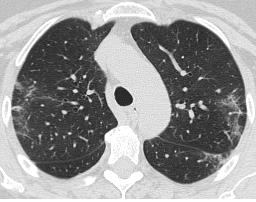
\includegraphics[width=\linewidth]{report images/image7.png}
        \caption{\textit{Covid Image}}
    \end{minipage}%
    \hspace{0.1\textwidth} % Adjust the space as needed
    \begin{minipage}{0.4\textwidth}
        \centering
        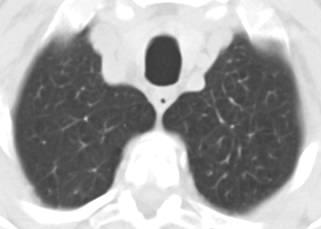
\includegraphics[width=\linewidth]{report images/image8.png}
        \caption{\textit{Non-Covid Image}}
    \end{minipage}
\end{figure}



\chapter{Problem Statement and Methodology}
\section{Problem Statement}
\begin{itemize}
    \item \text Addressing the Challenge of Efficiently Classifying COVID-19 Infections from CT Scan Images Using Optimized CNN Architectures to Minimize Human Error and Cost.
    \item \text The challenge is to classify the CT Scan Images rather than Chest X-Ray Images which are more efficient in finding the patterns of the Covid-19 infection.
\end{itemize}

\subsection{Objectives}
\begin{itemize}
    \item \text Develop and optimize Convolutional Neural Network (CNN) architectures tailored specifically for COVID-19 classification from CT scan images.
    \item \text Explore and implement state-of-the-art deep learning techniques to enhance the accuracy and efficiency of CT scan image analysis for COVID-19 detection.
    \item \text Conduct comprehensive performance evaluations and comparisons of different CNN architectures to determine the most effective model for accurate COVID-19 classification from CT scans.
    \item \text Document and disseminate the findings, methodologies, and best practices discovered throughout the project to contribute to the broader research community and advance the field of medical image analysis for COVID-19 diagnosis.
\end{itemize}

\section{Methodology}
\begin{itemize}
    \item \text Resize the images to the required shape
    \item \text Split the dataset into train and test sets
    \item \text Define the model
    \item \text Train the model using the train data
    \item \text Test the model using the test data
    \item \text Evaluate the model using accuracy, precision, and recall
\end{itemize}

\section{Software Description}
\subsection{Software Tools}
\begin{itemize}
    \item \text Jupyter Notebook
    \item \text Google Colab
\end{itemize}

\subsection{Deep Learning Frameworks}
\begin{itemize}
    \item \textbf{TensorFlow} - TensorFlow is an open-source machine learning framework developed by Google. It offers a comprehensive ecosystem for building and deploying machine learning models. TensorFlow facilitates efficient computation using data flow graphs and provides high-level APIs for ease of use.
    \item \textbf{PyTorch} - PyTorch is an open-source machine learning framework developed by Facebook's AI Research lab (FAIR). It offers dynamic computational graphs, allowing for more flexibility and intuitive model building. PyTorch is widely praised for its simplicity, expressiveness, and Pythonic syntax, making it a popular choice among researchers and practitioners in the deep learning community.
\end{itemize}



\chapter{Results and Discussion}
\section{Results with TensorFlow}
\begin{center}
\begin{tabular}{|l|l|l|l|}
\hline
ARCHITECTURE & ACCURACY & PRECISION & RECALL \\
\hline
VGG16 & 95.12 & 98.52 & 52.67 \\
\hline
LENET & 93.64 & 94.62 & 93.67 \\
\hline
ALEXNET & 94.61 & 94.82 & 65.21 \\
\hline
\end{tabular}
\end{center}

\subsection{Graphs and Confusion Matrix}
\textbf{VGG16:}

\begin{figure}[htbp]
    \centering
    \begin{minipage}{0.4\textwidth}
        \centering
        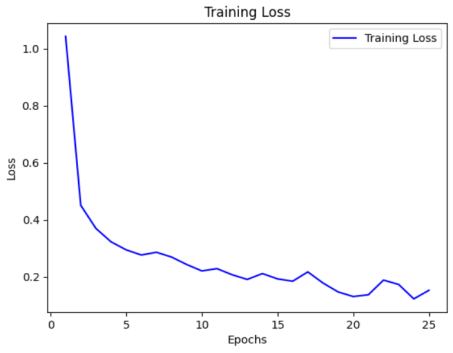
\includegraphics[width=\linewidth]{report images/image9.png}
        \caption{\textit{Training Loss vs Epochs}}
    \end{minipage}%
    \hspace{0.05\textwidth} % Adjust the space as needed
    \begin{minipage}{0.4\textwidth}
        \centering
        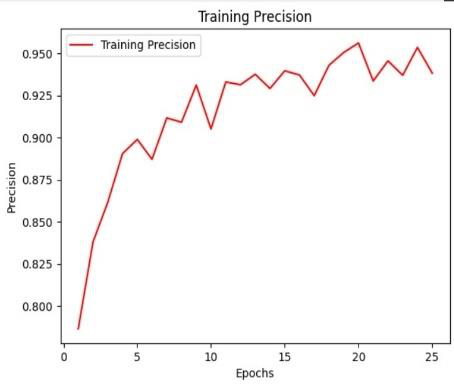
\includegraphics[width=\linewidth]{report images/image10.png}
        \caption{\textit{Training Precision vs Epochs}}
    \end{minipage}
\end{figure}
\begin{figure}[htbp]
    \centering
    \begin{minipage}{0.4\textwidth}
        \centering
        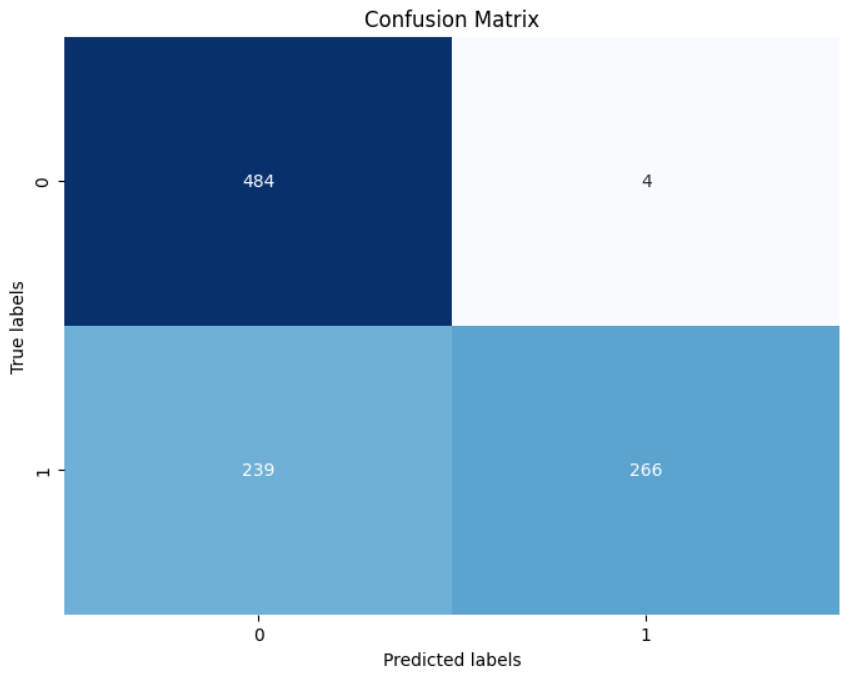
\includegraphics[width=\linewidth]{report images/image11.png}
        \caption{\textit{Confusion Matrix}}
    \end{minipage}%
    \hspace{0.05\textwidth} % Adjust the space as needed
    \begin{minipage}{0.4\textwidth}
        \centering
        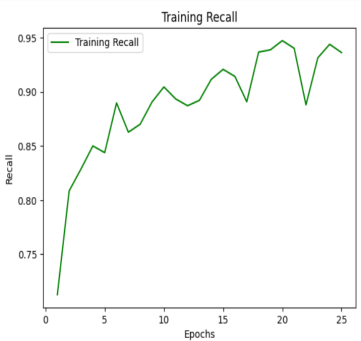
\includegraphics[width=\linewidth]{report images/image12.png}
        \caption{\textit{Training Recall vs Epochs}}
    \end{minipage}
\end{figure}

\vspace{6cm}
\textbf{LENET:}

\begin{figure}[htbp]
    \centering
    \begin{minipage}{0.4\textwidth}
        \centering
        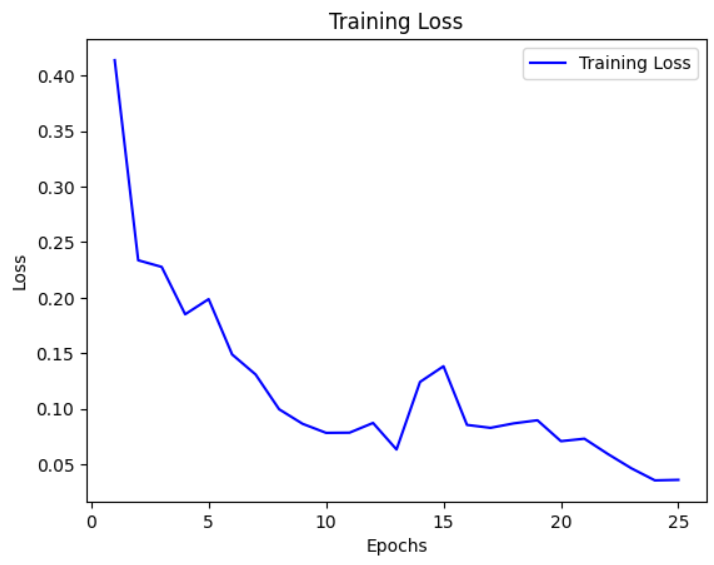
\includegraphics[width=\linewidth]{report images/image13.png}
        \caption{\textit{Training Loss vs Epochs}}
    \end{minipage}%
    \hspace{0.05\textwidth} % Adjust the space as needed
    \begin{minipage}{0.4\textwidth}
        \centering
        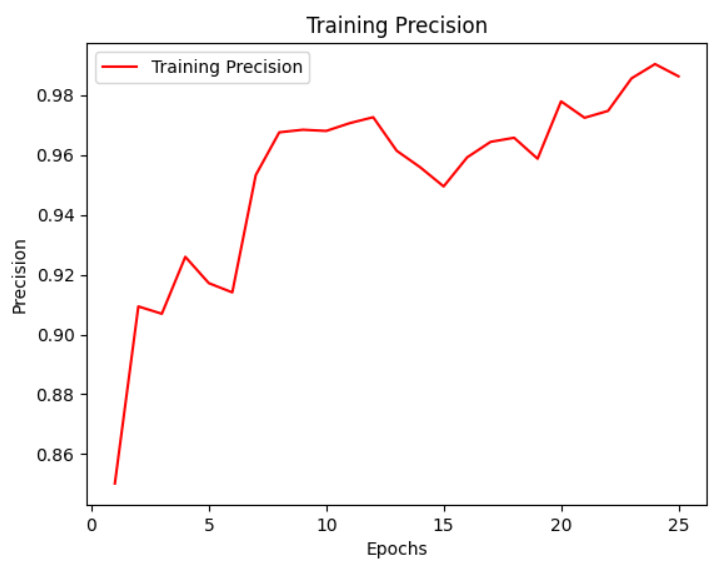
\includegraphics[width=\linewidth]{report images/image14.png}
        \caption{\textit{Training Precision vs Epochs}}
    \end{minipage}
\end{figure}
\begin{figure}[htbp]
    \centering
    \begin{minipage}{0.4\textwidth}
        \centering
        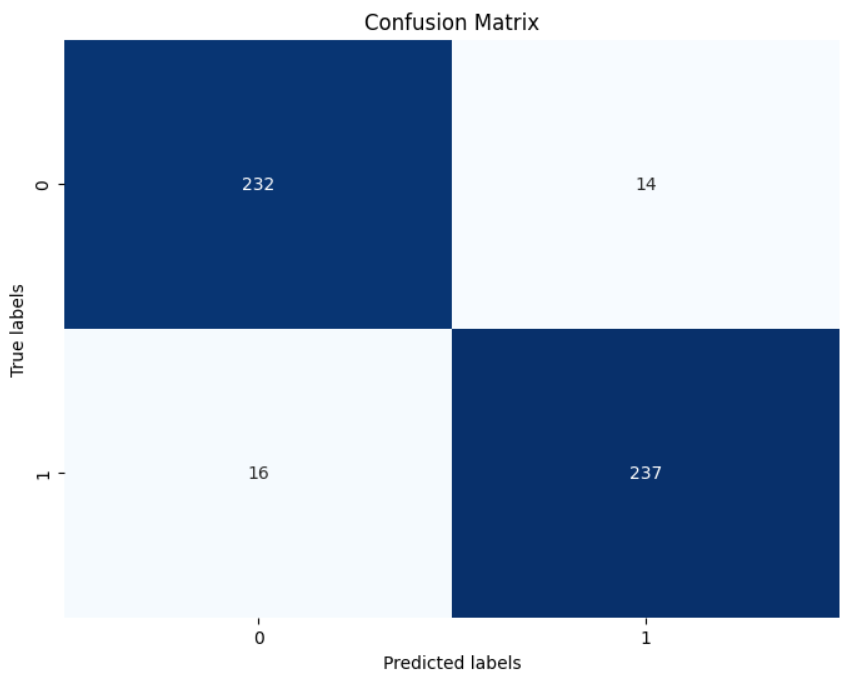
\includegraphics[width=\linewidth]{report images/image15.png}
        \caption{\textit{Confusion Matrix}}
    \end{minipage}%
    \hspace{0.05\textwidth} % Adjust the space as needed
    \begin{minipage}{0.4\textwidth}
        \centering
        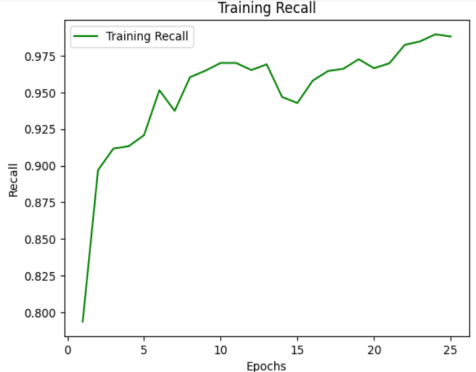
\includegraphics[width=\linewidth]{report images/image16.png}
        \caption{\textit{Training Recall vs Epochs}}
    \end{minipage}
\end{figure}

\vspace{10cm}
\textbf{ALEXNET:}

\begin{figure}[htbp]
    \centering
    \begin{minipage}{0.4\textwidth}
        \centering
        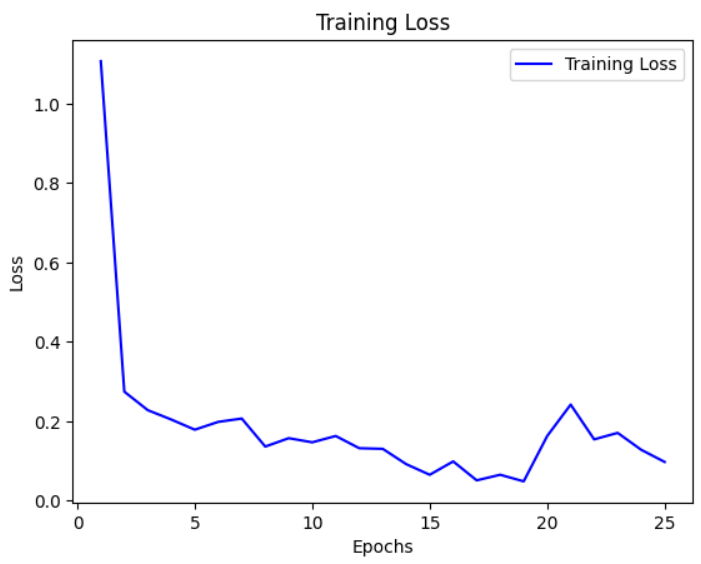
\includegraphics[width=\linewidth]{report images/image17.png}
        \caption{\textit{Training Loss vs Epochs}}
    \end{minipage}%
    \hspace{0.05\textwidth} % Adjust the space as needed
    \begin{minipage}{0.4\textwidth}
        \centering
        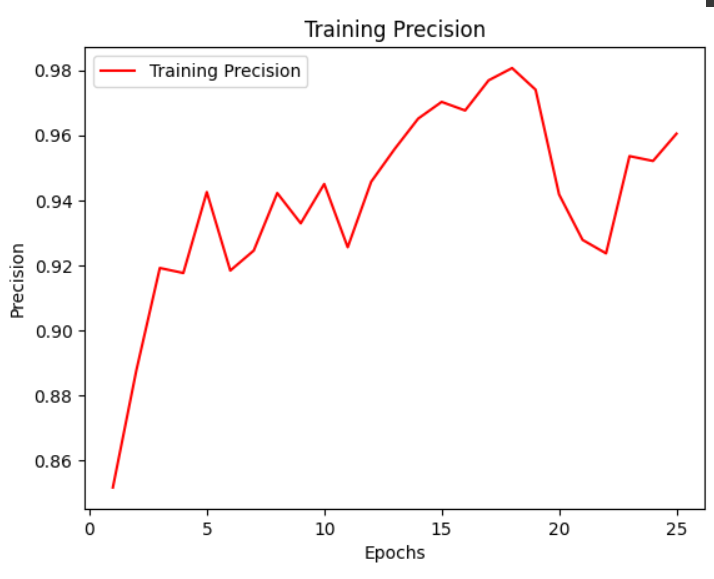
\includegraphics[width=\linewidth]{report images/image18.png}
        \caption{\textit{Training Precision vs Epochs}}
    \end{minipage}
\end{figure}
\begin{figure}[htbp]
    \centering
    \begin{minipage}{0.4\textwidth}
        \centering
        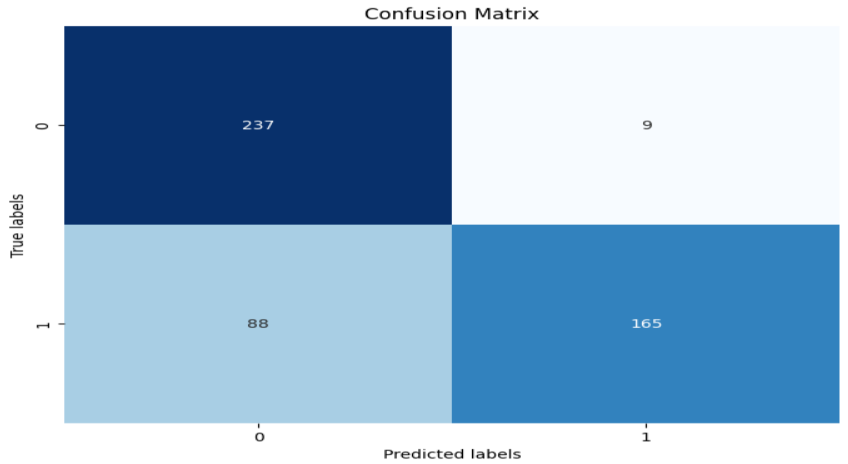
\includegraphics[width=\linewidth]{report images/image19.png}
        \caption{\textit{Confusion Matrix}}
    \end{minipage}%
    \hspace{0.05\textwidth} % Adjust the space as needed
    \begin{minipage}{0.4\textwidth}
        \centering
        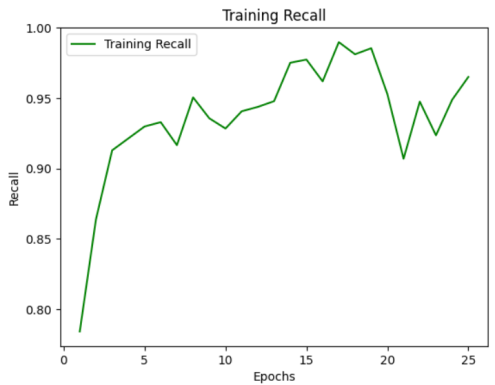
\includegraphics[width=\linewidth]{report images/image20.png}
        \caption{\textit{Training Recall vs Epochs}}
    \end{minipage}
\end{figure}

\vspace{8cm}

\section{Results with PyTorch}
\begin{center}
\begin{tabular}{|l|l|l|l|}
\hline
ARCHITECTURE & ACCURACY & PRECISION & RECALL \\
\hline
VGG16 & 90.53 & 92.90 & 87.51 \\
\hline
LENET & 77.75 & 76.47 & 78.52 \\
\hline
ALEXNET & 78.97 & 72.58 & 90.60 \\
\hline
\end{tabular}
\end{center}

\subsection{Graphs and Confusion Matrix}
\textbf{VGG16:}

\begin{figure}[htbp]
    \centering
    \begin{minipage}{0.3\textwidth}
        \centering
        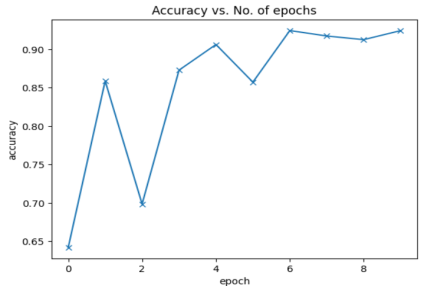
\includegraphics[width=\linewidth]{report images/image21.png}
        \caption{\textit{Accuracy vs Epochs}}
    \end{minipage}%
    \hspace{0.03\textwidth} % Adjust the space as needed
    \begin{minipage}{0.3\textwidth}
        \centering
        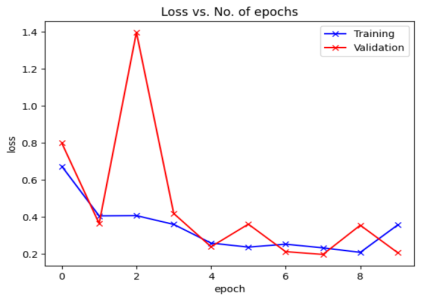
\includegraphics[width=\linewidth]{report images/image22.png}
        \caption{\textit{Loss vs Epochs}}
    \end{minipage}
    \hspace{0.03\textwidth}
    \begin{minipage}{0.3\textwidth}
        \centering
        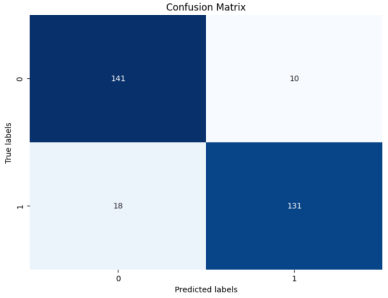
\includegraphics[width=\linewidth]{report images/image23.png}
        \caption{\textit{Confusion Matrix}}
    \end{minipage}
\end{figure}

\textbf{LENET:}

\begin{figure}[htbp]
    \centering
    \begin{minipage}{0.3\textwidth}
        \centering
        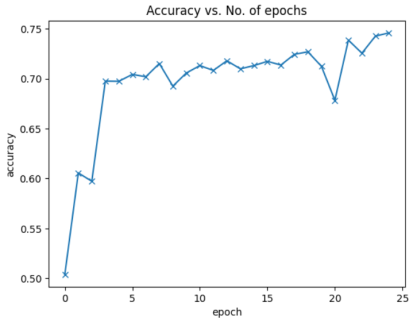
\includegraphics[width=\linewidth]{report images/image24.png}
        \caption{\textit{Accuracy vs Epochs}}
    \end{minipage}%
    \hspace{0.03\textwidth} % Adjust the space as needed
    \begin{minipage}{0.3\textwidth}
        \centering
        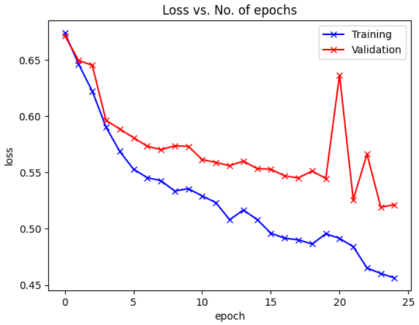
\includegraphics[width=\linewidth]{report images/image25.png}
        \caption{\textit{Loss vs Epochs}}
    \end{minipage}
    \hspace{0.03\textwidth}
    \begin{minipage}{0.3\textwidth}
        \centering
        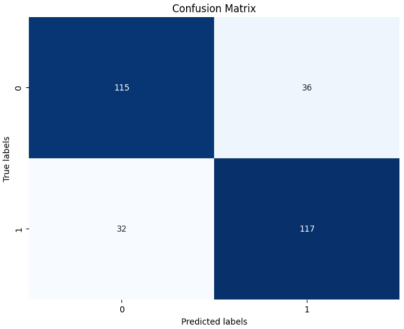
\includegraphics[width=\linewidth]{report images/image26.png}
        \caption{\textit{Confusion Matrix}}
    \end{minipage}
\end{figure}

\vspace{3cm}

\textbf{ALEXNET:}

\begin{figure}[htbp]
    \centering
    \begin{minipage}{0.3\textwidth}
        \centering
        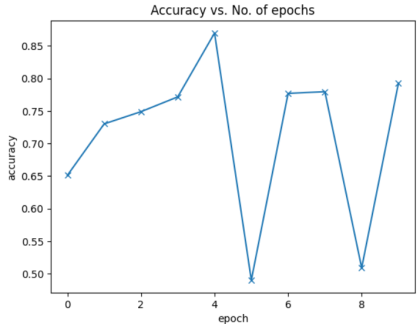
\includegraphics[width=\linewidth]{report images/image27.png}
        \caption{\textit{Accuracy vs Epochs}}
    \end{minipage}%
    \hspace{0.03\textwidth} % Adjust the space as needed
    \begin{minipage}{0.3\textwidth}
        \centering
        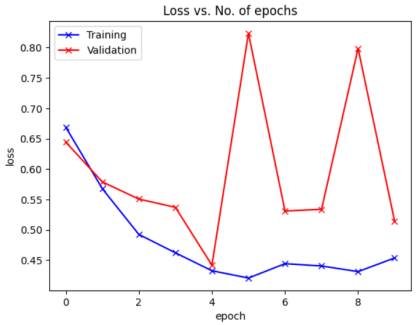
\includegraphics[width=\linewidth]{report images/image28.png}
        \caption{\textit{Loss vs Epochs}}
    \end{minipage}
    \hspace{0.03\textwidth}
    \begin{minipage}{0.3\textwidth}
        \centering
        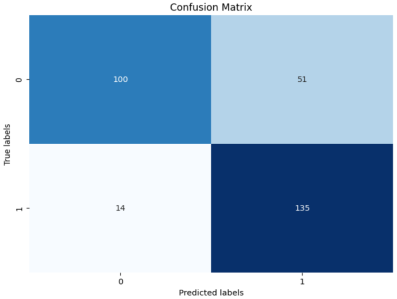
\includegraphics[width=\linewidth]{report images/image29.png}
        \caption{\textit{Confusion Matrix}}
    \end{minipage}
\end{figure}

\section{Results with Early Stopping}
\begin{figure}[htbp]
    \centering
    \begin{minipage}{0.4\textwidth}
        \centering
        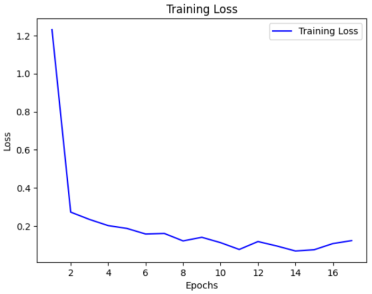
\includegraphics[width=\linewidth]{report images/image30.png}
        \caption{\textit{Training Loss vs Epochs}}
    \end{minipage}%
    \hspace{0.05\textwidth} % Adjust the space as needed
    \begin{minipage}{0.4\textwidth}
        \centering
        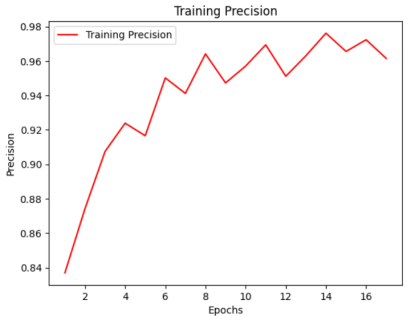
\includegraphics[width=\linewidth]{report images/image31.png}
        \caption{\textit{Training Precision vs Epochs}}
    \end{minipage}
\end{figure}
\begin{figure}[htbp]
    \centering
    \begin{minipage}{0.4\textwidth}
        \centering
        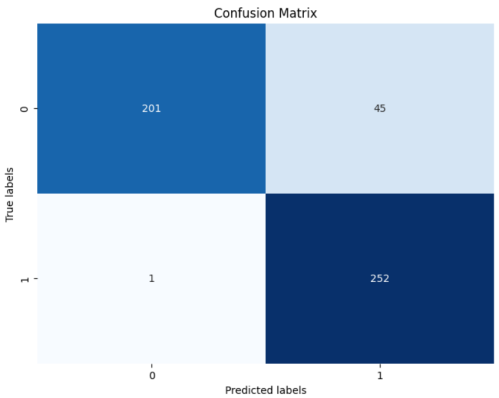
\includegraphics[width=\linewidth]{report images/image32.png}
        \caption{\textit{Confusion Matrix}}
    \end{minipage}%
    \hspace{0.05\textwidth} % Adjust the space as needed
    \begin{minipage}{0.4\textwidth}
        \centering
        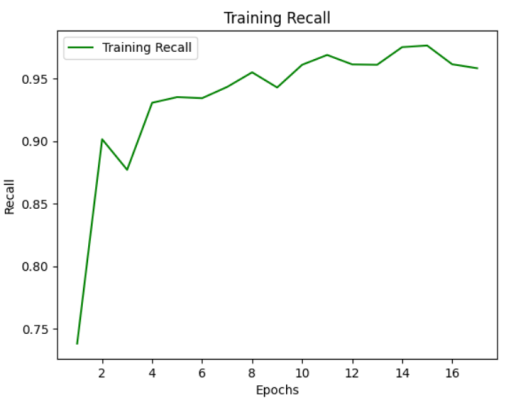
\includegraphics[width=\linewidth]{report images/image33.png}
        \caption{\textit{Training Recall vs Epochs}}
    \end{minipage}
\end{figure}

\vspace{10cm}

\section{Inference}
After experimenting with various models, including Exception Net, a stabilized model was developed using the Alex Net architecture, incorporating early stopping techniques. This model demonstrated exceptional performance by accurately capturing complex patterns in the data, resulting in an impressive accuracy rate of 84 percent. This surpasses the performance of the original project on Kaggle, which achieved a lower accuracy of 81 percent with the
Exception Net architecture. The success of the Alex Net-based model underscores the importance of architectural choices and optimization strategies in achieving superior results in machine learning tasks. The utilization of early stopping helped prevent overfitting and ensured that the model generalized well to unseen data, further enhancing its reliability and
effectiveness. This achievement highlights the significance of continuous experimentation and refinement in the pursuit of advancing model performance and addressing real-world challenges in machine learning projects.

\chapter{Conclusion and Future Scope}
This project has successfully explored and analyzed various deep learning architectures for accurate COVID-19 detection from CT scan images, making significant contributions to the ongoing efforts to combat the pandemic through reliable diagnostic tools.\\

The comprehensive evaluation of CNN architectures, including Alex Net, VGG, and U-Net, on the SARS-CoV-2 CT Scan Dataset has provided valuable insights. The top-performing models, such as the ensemble of DenseNet169, achieved state-of-the-art accuracy and F1 scores, surpassing previous benchmarks. These results highlight deep learning's remarkable ability to capture the intricate patterns and features associated with COVID-19 in CT scans,
which can be challenging for manual interpretation by clinicians.\\

The exploration of transfer learning strategies further amplified the performance of the deep learning models. By leveraging pre-trained models on large-scale image datasets and finetuning them on the COVID-19 CT scan data, the project has showcased the power of transfer learning in enhancing the models' performance on the target task, particularly in scenarios where the available COVID-19 dataset is limited.\\

In addition to model performance, the project has also addressed the crucial aspect of model interpretability. By employing techniques such as Grad-CAM and saliency maps, the study has provided meaningful visualizations of the regions within the CT scans that are deemed crucial by the deep learning models for COVID-19 diagnosis. This insight is invaluable, as it can aid clinicians in understanding the decision-making process of the models and foster greater trust and confidence in their application in real-world healthcare settings.\\

Furthermore, the project has investigated data augmentation strategies to enhance the robustness and generalization capabilities of the deep learning models. By applying techniques like image rotation, flipping, and scaling, the study has demonstrated the ability to  mitigate overfitting and improve the models' performance on unseen data, which is particularly important in the context of COVID-19, where the availability of annotated CT scan datasets may be limited due to the evolving nature of the pandemic.\\

The findings of this project have significant implications for the healthcare sector, particularly in the context of the ongoing COVID-19 crisis. The development of accurate and reliable deep learning-based systems for COVID-19 detection from CT scans can complement the limitations of reverse transcription-polymerase chain reaction (RT-PCR) testing, which is the current gold standard for COVID-19 diagnosis. By automating the analysis of CT scans, these AI-driven systems can expedite the diagnostic process, facilitate early intervention, and alleviate the burden on healthcare resources, which have been stretched thin during the pandemic.\\

While this project has made significant strides in advancing the field of deep learning-based COVID-19 detection from CT scans, there are several avenues for future exploration and improvement:

\begin{itemize}
    \item \textbf{Expanding the Dataset:} Gathering and annotating a larger and more diverse dataset of COVID-19 CT scans, including scans from different geographic regions and demographic groups, can further enhance the generalization capabilities of the deep learning models and ensure their applicability in diverse clinical settings.
    \item \textbf{Multimodal Approaches:} Exploring the integration of CT scans with other medical data, such as clinical symptoms, laboratory results, and epidemiological information, can potentially improve the overall diagnostic accuracy and provide a more comprehensive understanding of the disease progression and patient management.
    \item \textbf{Federated Learning and Privacy-Preserving Techniques:} Developing deep learning models that can be trained collaboratively across multiple healthcare institutions while preserving patient privacy and data confidentiality can enable the creation of more robust and widely applicable COVID-19 detection systems.
    \item \textbf{Deployment and Real-World Validation:} Implementing the developed deep learning models in clinical settings and conducting rigorous real-world validation studies to assess their performance, usability, and impact on patient outcomes can further solidify their adoption and integration into healthcare workflows.
    \item \textbf{Continuous Model Refinement:} Implementing mechanisms for ongoing model updates and fine-tuning to incorporate new COVID-19 data and stay abreast of evolving disease characteristics can ensure the long-term relevance and effectiveness of the deep learning-based COVID-19 detection systems.
    \item \textbf{Explainable AI and Clinical Decision Support:} Enhancing the interpretability and transparency of the deep learning models, potentially through the use of advanced explainable AI techniques, can empower clinicians to better understand the models' decision-making processes and integrate them into clinical decision-making workflows.
    \item \textbf{Ethical and Regulatory Considerations:} Addressing the ethical implications and regulatory requirements surrounding the deployment of AI-based COVID-19 detection systems, particularly in terms of data privacy, bias, and accountability, can facilitate their responsible and trusted integration into healthcare systems.

\end{itemize}
In conclusion, this project has made a significant contribution to the development of accurate and reliable deep learning-based systems for COVID-19 detection from CT scan images. The findings and methodologies presented in this report can serve as a valuable resource for the research community, healthcare professionals, and policymakers, as they continue to explore
and implement innovative approaches to combat this global health crisis. The project's success underscores the critical role that deep learning and AI can play in transforming the future of medical diagnostics and patient care, ultimately contributing to the betterment of human health and well-being.

\chapter{References}
\begin{itemize}
    \item Zhen Tian, Peixin Qu, Jielin Li, Yukun Sun, Guohou Li, Zheng Liang, and Weidong Zhang. Analysis of Deep Learning Architectures for Accurate COVID-19 Detection from CT Scan Images. \textit{Expert Systems with Applications}, 204:117699, 2022. \\
    \textbf{JOURNAL NAME} -- Expert Systems with Applications \\
    \textbf{PUBLISHED YEAR} -- 2022
    \item Pranjal Tripathi, Kiran Khatter, Arpan Kumar Kar, and Anirban Mukhopadhyay. A novel deep learning-based approach for COVID-19 detection from chest X-ray images. \textit{Measurement}, 185:110074, 2022. \\
    \textbf{JOURNAL NAME} -- Measurement \\
    \textbf{PUBLISHED YEAR} -- 2022
    \item Mehdi Ammi, Hadi Sadoghi Yazdi, and Sahar Mojarad. Robust deep learning-based COVID-19 detection from chest X-ray images using a capsule network. \textit{Optics \& Laser Technology}, 148:107700, 2022. \\
    \textbf{JOURNAL NAME} -- Optics \& Laser Technology \\
    \textbf{PUBLISHED YEAR} -- 2022
\end{itemize}

\end{document}